% Contains the significance of the study and related literature.
%
%
%
\section{SIGNIFICANCE OF THE STUDY}
Behavioral analytics has recently emerged as a practice for commercial game development. These also relates to technological advancements brought about by mobile devices that enable developers to gather more significant data through the use of commercial analytics.

There is a significant increase on the number of games that are shifting to the free-to-play (F2P) model and this study are one of the few instances wherein commercial game dataset are used for academic research. Findings will be beneficial for game companies that strictly complies with the F2P model. In specific, those who greatly rely on high user activity for their games will strongly find this paper beneficial for their business decisions.

We present a novel approach on how analysts or developers may attempt to predict the DAU value on a practical scenario, based from the formula given by our prediction model. We also attempt to define features that are highly important based from our analysis of attributes on our dataset and as supported by other similar study as seen in \cite{ref:predicting_player_churn}.

In this manner, we present the following contributions in this paper:
We formally define from related study, as well as our findings,  the attributes that affects the DAU value.
We attempt to create several prediction models for the DAU value using machine learning techniques and explain its significance on a practical setting.
We present a simple method on how one can predict the DAU value
This paper are one of the few research study that uses dataset from commercial games which is otherwise, confidential and unavailable for academic research.
Despite a small number of installs for both games, Jungle Cubes have very strongly correlated attributes against DAU, which make the dataset significant. We present this in detail in the succeeding sections.

\subsection{Related Work}
Using game analytics for research purposes has recently been pursued around 2012.  Analysis of user behavior in digital games has become a fundamental practice for game companies. It is also open for numerous research opportunities due to its complex nature of modelling users while also taking into consideration the elements of the game. Thus, datasets concerning player behavior can be exceptionally complex like seen in World of Warcraft, a famous MMORPG (Massively Multiplayer Online Role-Playing Game), which has lead a team of researchers attempt to cluster players based from behavioral telemetry \cite{ref:player_clustering_wow}. They applied numerous unsupervised learning methods to discover clusters of "player groups" based from their playtime data and their levelling pace.

\subsubsection{Determining How Players Lose Interest}
A study on action and shooter games released on Playstation 3, that uses player behavior dataset, have been used to discover how players lose interest in playing a game \cite{ref:how_players_lose_interest}. The dataset presented in their research paper were extracted from two single-player games (Just Cause 2, Tomb Raider: Underworld) and three multi-player games (Battlefield Bad Company 2, Medal of Honor, Crysis 2).  All datasets have been sampled using simple random sampling or extraction of data on a timeline where player activities are high or the game was newly released.

The interest of playing a game cannot be measured directly but can be inferred from observable data as mentioned by \cite{ref:how_players_lose_interest}. In reality, a player's urge to play a game is influenced by several factors that appears as unforeseeable events to the analysts involved. This ranges from variance in playing schedules, personal satisfaction, release of new game content, or new games that competes with the player's attention. Using these consideration as mentioned by \cite{ref:how_players_lose_interest}, they modeled the player's interest in playing a game as a random process. That is, at any given time, a player's interest is a random quantity that may or may not depend on previous values and future values cannot be predicted exactly. Thus, they have restricted their mathematical models to random process models; the Gamma distribution, Weibull distribution, Inverse Gaussian distribution, and Log-normal distribution.

Of all five games analyzed, researchers deduced that the total playing times follows the Weibull distribution. Following the Weibull model, it gives a good benchmark for gaming companies to determine how a player's playtime even before the game has been released.

\subsubsection{Predicting Churn Rate}
There is an existing research work that is highly related to our methodology. Researchers attempted to predict the Churn Rate of commercial mobile games which also uses some attributes we use for this study \cite{ref:predicting_player_churn}. In their study, they threat the churn value as a binary classification task, a player is labelled as \textbf{churned} or \textbf{returning}. Given a specified \textit{cutoff date}, the player will be labelled as \textbf{churned} or \textbf{returning} based from two formal problems defined in their study.

They described problem \textbf{P1} to be more straightforward. Given a cutoff date, players who did not return after the cutoff date are immediately considered as churners. The green dots in \ref{fig:churn_figure} are considered as \textbf{churners} while the red dots are players who managed to return after the specified cutoff date. This formal definition of churn is harsh and not useful for real-world applications. Problem \textbf{P2} is more relaxed. Given a grace period after the specified cutoff date, if players return during this period, they are considered as "about to churn" wherein their engagement to the game is already low. These are the players who are likely to quit soon and knowing how much players are inside this grace period aids gaming companies on potentially rescuing these players to get back to the game. In \ref{fig:churn_figure}, the first two green dots refer to players already churned while the third green dot inside the grace period is flagged as "about to churn." The red dot is a player who managed to return to the game after the grace period.

Figure \ref{fig:churn_figure} shows an illustration of formal problem \textbf{P1} and problem \textbf{P2}.

\begin{figure*}[h]
\centering
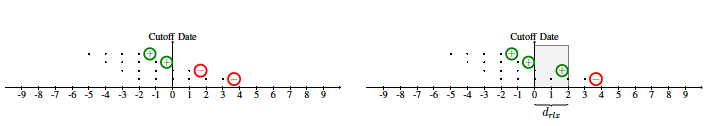
\includegraphics[scale=0.6]{figures/churn.png}
\caption{Formal problems defined as \textbf{P1} and \textbf{P2} described by \cite{ref:predicting_player_churn}. \textbf{P1} defines users as churners if they do not return after the specified cutoff date. In \textbf{P2}, players are given a grace period after the cutoff date. If players did not return after the specified grace period, they are considered as churners. }
\label{fig:churn_figure}
\end{figure*}


\begin{itemize}
\item Feature Selection \\
Attributes were universal and game-content independent. The following attributes stood out based from their feature selection tests and obvious observations that affect churning behavior; \textbf{Number of Sessions}, \textbf{Number of Days}, \textbf{Current Absence Time}, \textbf{Playtime per Session}, and \textbf{Average Time Between Sessions} and \textbf{Predefined Spending Category}. Some of these attributes are observed in our study.

\item Experiments and Results \\
In their research work, the  most accurate classifier is the decision tree, among other different classifiers; neural networks, logistic regression, and naive bayes. F1-score goes as high as 0.916 for the decision tree model. We will also be using decision trees for our prediction since it has achieved a high accuracy from this study.
\end{itemize}


